\section{Preliminary results}

\begin{frame}{Library Size}
  \begin{columns}
    \begin{column}{0.5\textwidth}
      \begin{itemize}
        \item Execution time increases dramatically with library size due to combinatorial explosion.
        \item Same trend for number solutions, with more than 10 000 solutions for a library of 30 sub-topologies.
      \end{itemize}
    \end{column}
    \begin{column}{0.5\textwidth}
      \begin{figure}
        \centering
        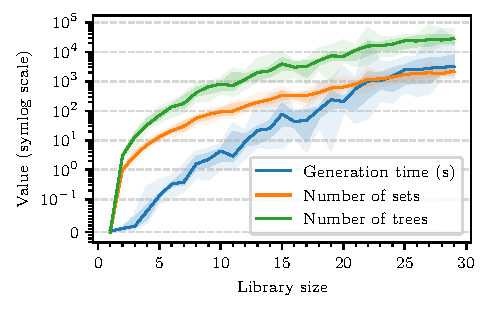
\includegraphics[width=\linewidth]{figures/feditn/results/library_size}
        \caption{Influence of the library size on generation.}
      \end{figure}
    \end{column}
  \end{columns}
\end{frame}


\begin{frame}{Number of Nodes}
  \begin{columns}
    \begin{column}{0.5\textwidth}
      \begin{itemize}
        \item All metrics increase exponentially with the number of nodes.
        \item Maximum number of nodes influences the cardinality of generated sets and tree compositions.
        \item No solutions exist for fewer than 4 nodes (library constraint).
      \end{itemize}
    \end{column}
    \begin{column}{0.5\textwidth}
      \begin{figure}
        \centering
        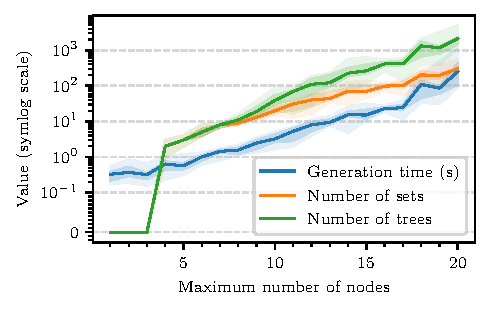
\includegraphics[width=\linewidth]{figures/feditn/results/max_nodes}
        \caption{Influence of the number of nodes on generation.}
      \end{figure}
    \end{column}
  \end{columns}
\end{frame}


\begin{frame}{Tree Depth}
  \begin{columns}
    \begin{column}{0.5\textwidth}
      \begin{itemize}
        \item Both metrics increase rapidly with tree depth, plateauing at depth 4 due to other constraints.
        \item High result variation is due to random sampling of sub-topologies.
      \end{itemize}
    \end{column}
    \begin{column}{0.5\textwidth}
      \begin{figure}
        \centering
        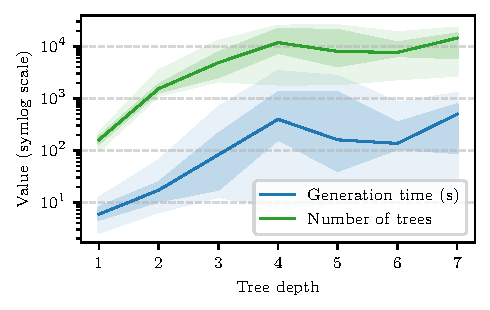
\includegraphics[width=\linewidth]{figures/feditn/results/tree_depth}
        \caption{Influence of tree depth on generation.}
      \end{figure}
    \end{column}
  \end{columns}
\end{frame}


\begin{frame}{Service Constraints}
  \begin{columns}
    \begin{column}{0.5\textwidth}
      \begin{itemize}
        \item Negative correlation between number of service constraints and sets/trees.
        \item Execution time remains nearly constant, as constraints are handled by pruning incompatible sets.
        \item Quickly conflicts with other constraints.
      \end{itemize}
    \end{column}
    \begin{column}{0.5\textwidth}
      \begin{figure}
        \centering
        \vspace{-1em}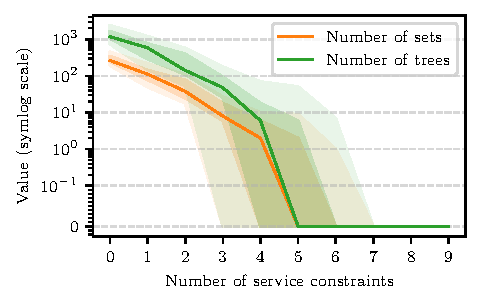
\includegraphics[width=0.8\linewidth]{figures/feditn/results/services_numbers}
        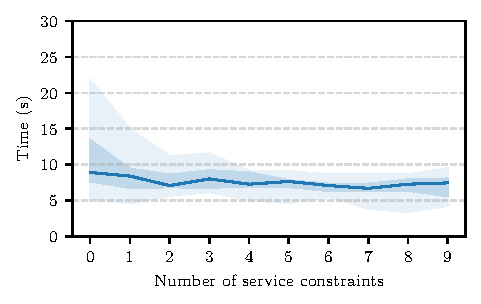
\includegraphics[width=0.8\linewidth]{figures/feditn/results/services_time}
        \vspace{-1em}\caption{Influence of the number of service constraints on generation.}
      \end{figure}
    \end{column}
  \end{columns}
\end{frame}